%%%%%%%%%%%%%%%%%%%%%%%%%%%%%%%%%%%%%%%%%%%%%%%%%%%%%%%%%%%%%%%%%%%%%%%
% file
% bismon/talks/Lamsade-21nov2019/Bismon-Starynkevitch-Lamsade-21nov2019.tex
% in http://github.com/bstarynk/bismon/
% inspired by http://cse.unl.edu/~cbourke/latex/UNLTheme.tex
%%%%%%%%%%%%%%%%%%%%%%%%%%%%%%%%%%%%%%%%%%%%%%%%%%%%%%%%%%%%%%%%%%%%%%%

\documentclass[xcolor=svgnames,final,smaller,a4]{beamer}
\usepackage{relsize}
\usepackage{luacode}
\usepackage{xcolor}
\usepackage{alltt}
\usepackage{wasysym}
\usepackage{listings}
\usepackage{hyperref}


\hypersetup{
  colorlinks   = true, %Colours links instead of ugly boxes
  urlcolor     = NavyBlue, %Colour for external hyperlinks
  linkcolor    = DarkGreen, %Colour of internal links
  citecolor   = DarkMagenta, %Colour of citations
  frenchlinks = true,
}

\usetheme[hideothersubsections]{Bismon}



\title{\textsc{Bismon} \\
a static source code analysis framework using \textit{some} symbolic artificial intelligence techniques.}
\author[B.Starynkevitch]{Basile \textsc{Starynkevitch} - \href{http://starynkevitch.net/Basile/}{\texttt{starynkevitch.net/Basile}}\\
  \href{mailto:basile.starynkevitch@cea.fr}{\color{blue}{\texttt{basile.starynkevitch@cea.fr}}} and \href{mailto:basile@starynkevitch.net}{\color{blue}{\texttt{basile@starynkevitch.net}}}
} %
\institute{ \raisebox{0.4cm}{CEA/LIST (DILS) - laboratoire de Sûreté des Logiciels -} 
\includegraphics[scale=0.14]{CEA-LIST-logo}}
\date{November 21\textsuperscript{st}, 2019}

\begin{document}
 \begin{luacode*}
   local gitpip=io.popen("git log --no-color --format=oneline -1 --abbrev=16 --abbrev-commit -q | cut -d' ' -f1")
   gitid=gitpip:read()
   gitpip:close()
 \end{luacode*}
 \newcommand{\mygitid}{\luadirect{tex.print(gitid)}}
 \newcommand{\Bismon}{\href{https://github.com/bstarynk/bismon}{\textsc{Bismon}}}

%{% open a Local TeX Group
%\setbeamertemplate{sidebar}{}
 \begin{frame}
   
   
   \begin{relsize}{-1.5}
        \titlepage
        \textcolor{brown}{{\large \textbf{Opinions are only mines}} (not from  CEA or E.C.)}
        
        \begin{center}
         

          git \texttt{\mygitid}
        \end{center}
   \end{relsize}
\end{frame}
%}% end Local TeX Group


\section{Introduction}

\begin{frame}
    \frametitle{Introduction}
    \framesubtitle{funding}

    {\Bismon} is funded by two \href{https://ec.europa.eu/programmes/horizon2020/en}{Horizon 2020} research and innnovation actions:
    
    \begin{itemize}
    \item \href{https://www.chariotproject.eu/}{\textsc{Chariot}}, under Grant Agreement 780075.
      \item \href{http://decoder-project.eu/}{\textsc{Decoder}}, under Grant Agreement 824231.
    \end{itemize}

    So  {\Bismon} is European.

    \begin{center}
      
\includegraphics[width=0.15\textwidth]{Flag-of-Europe} \raisebox{0.4cm}[1pt][1pt]{(100\% funded by the European Commission)}.
    \end{center}
    
    \textcolor{brown}{{\large \textbf{Opinions are only mines}} (not from  CEA or E.C.)}
    
\end{frame}
    
\begin{frame}
    \frametitle{Introduction}
    \framesubtitle{AI and other inspirations}

    \begin{itemize}

    \item D.Lenat work on \textsc{Rll -1} then \textsc{Eurisko}
    \item J.Pitrat\textsuperscript{\dag} {\relsize{-1}{(1934 - october 2019)}}
      \href{http://bootstrappingartificialintelligence.fr/WordPress3/}{pionneering
        work} on \href{http://starynkevitch.net/Basile/caia-su-24feb2016.tar.bz2}{\textsc{Caia}}
    \item my PhD work {\relsize{-1}{(1985 - 1990)}}
    \item my past \href{http://starynkevitch.net/Basile/gcc-melt/}{\textsc{Gcc Melt}} work {\relsize{-1}{(2008 - 2016)}}
    \item \href{http://frama-c.com/}{\textsc{Frama-C}}, its
      \href{https://frama-c.com/acsl_tutorial_index.html}{\textsc{Acsl}}, \href{http://ocaml.org}{\textsc{Ocaml}} runtime,
      and \textit{non-relational} databases
    \item \href{http://gcc.gnu.org/}{\textsc{Gcc}}  $> 10$MLOC of \textit{C++} {\relsize{-1}{(bootstrapped with \texttt{g++ -O2 -flto})}}
 and a dozen of \href{https://en.wikipedia.org/wiki/Domain-specific_language}{DSL}s
    \end{itemize}

    For references, see the \href{http://starynkevitch.net/Basile/bismon-chariot-doc.pdf}{{\Bismon} \textbf{draft} report} on \href{http://starynkevitch.net/Basile/}{my home page}

    Some \href{https://www.gnu.org/licenses/gpl-3.0.en.html}{GPLv3+} code for \textsc{Linux/x86-64} desktop is available
    \href{http://github.com/bstarynk/bismon}{\texttt{github.com/bstarynk/bismon}}

    \hrule
    
    These slides are under \href{https://creativecommons.org/licenses/by-sa/4.0/}{
\includegraphics[scale=0.75]{CC-BY-SA-4}} \relsize{-1}{(CC-BY-SA-4)} and available from \href{http://starynkevitch.net/Basile/Bismon-Starynkevitch-Lamsade-21nov2019.pdf}{\texttt{starynkevitch.net/Basile/Bismon-Starynkevitch-Lamsade-21nov2019.pdf}}

    
    
\end{frame}

\begin{frame}
    \frametitle{Introduction}
    \framesubtitle{motivations}

    \textbf{Help} small teams of mostly \emph{junior} software developers (e.g. IoT) using \textsc{Linux} thru a collaborative \textit{Web} \emph{assistant} tool

    \begin{center}
      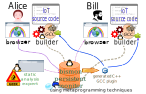
\includegraphics[width=0.90\textwidth]{bismon-monitor}
    \end{center}
    
\end{frame}
%%%%%%%%%%%%%%%%%%%%%%%%%%%%%%%%%%%%%%%%%%%%%%%%%%%%%%%%%%%%%%%%


\section{Data and persistence}

\begin{frame}
    \frametitle{Data and persistence}
    \framesubtitle{the \emph{Bismon} heap \textbf{\large greatly simplified} {\relsize{-1}{(my figure borrowed from \href{http://refpersys.org/}{\texttt{refpersys.org}})}}}

    \begin{center}
      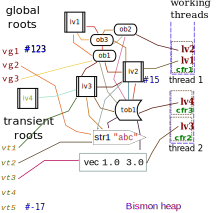
\includegraphics[width=0.72\textwidth]{heap-bismon}
    \end{center}
\end{frame}

\begin{frame}
    \frametitle{Data and persistence}
    \framesubtitle{garbage-collected values in \Bismon}

    \begin{itemize}
    \item {\textcolor{red}{\textbf{immutable values}}}  {\relsize{-1}{(often with \href{https://en.wikipedia.org/wiki/Flexible_array_member}{flexible array members} in \textit{C} code)}} : \begin{itemize}
    \item scalar values: tagged 63 bits \textbf{integers}, boxed \textbf{strings}, boxed \textbf{doubles} {\relsize{-1}{(not \texttt{NaN}, since it is uncomparable)}} \ldots
    \item composite values : \begin{itemize}
    \item ordered \textbf{sets} of objects with $O(\log n)$ membership test
    \item sequential \textbf{tuples} of objects {\relsize{-1}{(same layout in memory as sets)}}
    \item \textbf{nodes} with an object connective and zero or more son values.
      \item \textbf{closures} with their code represented by an object, and zero or more closed values {\relsize{-1}{(same data layout as nodes)}}
    \end{itemize}
    \end{itemize}
    \item \textbf{mutable and lockable} so ``heavy'' \textbf{\textcolor{red}{objects}} {\relsize{-1}{(each having its \textit{unique objid} e.g. \texttt{\_5t7pTgRckFK\_7hOY5yvx8v3})}}
    \end{itemize}

    In addition, our GC manages \textbf{quasi-values} as an
    \textit{implementation detail}. A quasi-value is simply a GC-ed
    memory zone which could belong to some value or object.
\end{frame}

%%%%%%%%%%%%%%%%
\begin{frame}
    \frametitle{Data and persistence}
    \framesubtitle{garbage collection in \Bismon ~ (1/3)}

    {\href{http://gchandbook.org/}{\textcolor{red}{\textbf{Garbage
          collection}}}} is:
    \begin{itemize}
    \item well understood in theory but difficult in practice
    \item dealing with \textbf{whole-program properties} of running processes
    \item related to \textbf{virtual memory} and \textbf{virtual address space}
    \item \textcolor{purple}{\textbf{crucially important for performance}} : \begin{itemize}
    \item can be very efficient, at least with single-threaded mostly
      immutable values {\relsize{-1}{(see \textsc{Ocaml}, \textsc{Haskell},
      \href{http://sbcl.org/}{\textsc{Sbcl}} or some \textsc{Jvm} implementations)}}
      \item very brittle {\relsize{-1}{(a GC bug usually crashes your program)}}
    \end{itemize}
      
      \item practically very dependent of both hardware (CPU cache)
        and operating system.

        \item still an \textcolor{red}{\textbf{art of delicate trade-offs}} {\relsize{-1}{(finalizers, decaying or weak pointers, tuning parameters, size of generations, frequency of major GCs, ...)}}
        
    \end{itemize}
\end{frame}
%%%%%%%%%%%%%%%%
\begin{frame}
    \frametitle{Data and persistence}
    \framesubtitle{garbage collection in \Bismon ~ (2/3)}
    
    {\href{http://gchandbook.org/}{\textcolor{red}{\textbf{Garbage
            collection}}}} is:
    
    \begin{itemize}

     \item requiring boring coding conventions and calling conventions at runtime

     \item needing cooperation from the compiler or code generator

     \item depending upon compiler optimizations

     \item {\textcolor{red}{\textbf{difficult to code}}}, notably with multi-threading

     \item {\textcolor{red}{\textbf{difficult to debug and test}}} (\href{https://en.wikipedia.org/wiki/Heisenbug}{Heisenbugs})


      
     \item wanting {\textcolor{red}{\textbf{metaprogramming}}} {\relsize{-1}{(the code of GC support routines should be easily generated, since very regular and )}}

          \item using algorithms (in copying GCs) close to
            persistence, since traversing the entire heap graph.
            
   \end{itemize}
   
\end{frame}

%%%%%%%%%%%%%%%%
\begin{frame}
    \frametitle{Data and persistence}
    \framesubtitle{garbage collection in \Bismon ~ (3/3)}

    Today, in november 2019, it is :
    \begin{itemize}

    \item slow, bad but easy naive, precise, mark-and-sweep GC algorithm

    \item does not scale yet to large 50Gbytes heaps

    \item should be generated by metaprogramming

    \item multi-thread ``friendly'' \smiley{} : stop the world variety \textcolor{green}{(joke!)}
      
        \item a \textbf{design bug} in {\Bismon}
          {\href{https://github.com/bstarynk/bismon/commit/6b26b802b8c0f4dee3053afea9fe3ef6e3073dca}{commit
            \texttt{6b26b802b8c0f4dee3053}}} : \textsc{Gtk} recursive
          event loop breaking our GC invariants.
        \item should become a copying generational GC for immutable values, and a tri-color marking onne for mutable objects
        \item then the write-barrier has to be implemented by changing the metaprogram (i.e. our C code generator)
          \item \textbf{not \href{http://man7.org/linux/man-pages/man3/dlclose.3.html}{\texttt{dlclose}}-ing} generated plugins {\relsize{-1}{(still
            science-fiction but should be theoretically done for
            garbage collection of generated code)}}.

    \end{itemize}
\end{frame}

\end{document}
%%%%%%%%%%%%%%%%%%%%%%%%%%%%%%%%%%%%%%%%%%%%%%%%%%%%%%%%%%%%%%%%
%% Local Variables: ;;
%% compile-command: "./build.sh" ;;
%% End: ;;
%%%%%%%%%%%%%%%%%%%%%%%%%%%%%%%%%%%%%%%%%%%%%%%%%%%%%%%%%%%%%%%%
